%%%%%%%%%%%%%%%%%%%%%%%%%%%%%%%%%%%%%%%%%
% Beamer Presentation
% LaTeX Template
% Version 1.0 (10/11/12)
%
% This template has been downloaded from:
% http://www.LaTeXTemplates.com
%
% License:
% CC BY-NC-SA 3.0 (http://creativecommons.org/licenses/by-nc-sa/3.0/)
%
%%%%%%%%%%%%%%%%%%%%%%%%%%%%%%%%%%%%%%%%%

%----------------------------------------------------------------------------------------
%	PACKAGES AND THEMES
%----------------------------------------------------------------------------------------

\documentclass{beamer}

\mode<presentation> {

% The Beamer class comes with a number of default slide themes
% which change the colors and layouts of slides. Below this is a list
% of all the themes, uncomment each in turn to see what they look like.

%\usetheme{default}
%\usetheme{AnnArbor}
%\usetheme{Antibes} % sungsoo's favorite theme
%\usetheme{Bergen}
%\usetheme{Berkeley}
%\usetheme{Berlin}
%\usetheme{Boadilla}
%\usetheme{CambridgeUS}
%\usetheme{Copenhagen}
%\usetheme{Darmstadt}
%\usetheme{Dresden}
%\usetheme{Frankfurt} % sungsoo
%\usetheme{Goettingen}
%\usetheme{Hannover}
%\usetheme{Ilmenau}
%\usetheme{JuanLesPins}
%\usetheme{Luebeck}
\usetheme{Madrid}
%\usetheme{Malmoe}
%\usetheme{Marburg}
%\usetheme{Montpellier}
%\usetheme{PaloAlto}
%\usetheme{Pittsburgh}
%\usetheme{Rochester}
%\usetheme{Singapore}
%\usetheme{Szeged}
%\usetheme{Warsaw}

% As well as themes, the Beamer class has a number of color themes
% for any slide theme. Uncomment each of these in turn to see how it
% changes the colors of your current slide theme.

%\usecolortheme{albatross}
%\usecolortheme{beaver}
%\usecolortheme{beetle}
%\usecolortheme{crane}
%\usecolortheme{dolphin}
%\usecolortheme{dove}
%\usecolortheme{fly}
%\usecolortheme{lily}
%\usecolortheme{orchid}
%\usecolortheme{rose}
%\usecolortheme{seagull}
%\usecolortheme{seahorse}
%\usecolortheme{whale}
%\usecolortheme{wolverine}

%\setbeamertemplate{footline} % To remove the footer line in all slides uncomment this line
%\setbeamertemplate{footline}[page number] % To replace the footer line in all slides with a simple slide count uncomment this line

%\setbeamertemplate{navigation symbols}{} % To remove the navigation symbols from the bottom of all slides uncomment this line
}

\usepackage{times} 
\usepackage{graphicx} % Allows including images
\usepackage{booktabs} % Allows the use of \toprule, \midrule and \bottomrule in tables
\graphicspath{{images/}} % Location of the slide background and figure files

% ===============================================================
%    My Commands
    \newcommand{\bi}{\begin{itemize}}
    \newcommand{\ei}{\end{itemize}}
    \newcommand{\be}{\begin{enumerate}}
    \newcommand{\ee}{\end{enumerate}}
    \newcommand{\ii}{\item}
    \newtheorem{Def}{Definition}
    \newtheorem{Lem}{Lemma}

%------------------------------------------------
% Colors
\usepackage{xcolor}	 % Required for custom colors
% Define a few colors for making text stand out within the presentation
\definecolor{mygreen}{RGB}{44,85,17}
\definecolor{myblue}{RGB}{34,31,217}
\definecolor{mybrown}{RGB}{194,164,113}
\definecolor{myred}{RGB}{255,66,56}
% Use these colors within the presentation by enclosing text in the commands below
\newcommand*{\mygreen}[1]{\textcolor{mygreen}{#1}}
\newcommand*{\myblue}[1]{\textcolor{myblue}{#1}}
\newcommand*{\mybrown}[1]{\textcolor{mybrown}{#1}}
\newcommand*{\myred}[1]{\textcolor{myred}{#1}}
%------------------------------------------------

\newcommand{\encode}[1]{\left< #1 \right> }
\newcommand{\paren}[1]{\left( #1 \right) }
\newcommand{\setbrac}[1]{\left\{ #1 \right\} }
\newcommand{\brac}[1]{\left[ #1 \right]}

\newcommand{\ands}{\wedge}
\newcommand{\ors}{\vee}
\newcommand{\thens}{\to}
\newcommand{\iffs}{\leftrightarrow}
\newcommand{\nots}{\sim}
\newcommand{\fd}{\rightarrow}
\newcommand{\mvd}{\twoheadrightarrow}
\newcommand{\inter}{\cap}
\newcommand{\union}{\cup}
\newcommand{\select}{\sigma}
\newcommand{\diff}{-}
\newcommand{\project}{\pi}
\newcommand{\rename}{\rho}
\newcommand{\join}{\Join}
\newcommand{\Null}{\text{NULL}}

%----------------------------------------------------------------------------------------
%	TITLE PAGE
%----------------------------------------------------------------------------------------

%\title[Flying KIWI]{Approximate Query Processing in Flying KIWI} % The short title appears at the bottom of every slide, the full title is only on the title page
\title[\textit{Flying KIWI}]{Probabilistic Databases} % The short title appears at the bottom of every slide, the full title is only on the title page

\author{Sung-Soo Kim} % Your name
\institute[ETRI] % Your institution as it will appear on the bottom of every slide, may be shorthand to save space
{
\textit{sungsoo@etri.re.kr} \\ % Your email address
\medskip
Data Management Research Section, ETRI % Your institution for the title page
}
\date{\today} % Date, can be changed to a custom date

\begin{document}

\begin{frame}
\titlepage % Print the title page as the first slide
\end{frame}

\begin{frame}
\frametitle{References and Slide Credits}
\bi
\ii Dan Suciu et al, \textit{Probabilistic Databases}, Morgan \& Claypool Publishers, May 2011.
\ii Guy Van den Broeck, Dan Suciu, \textit{Lifted Probabilistic Inference in Relational Models}, Tutorial UAI 2014, 2014.
\ei

\begin{figure}[h]
\centering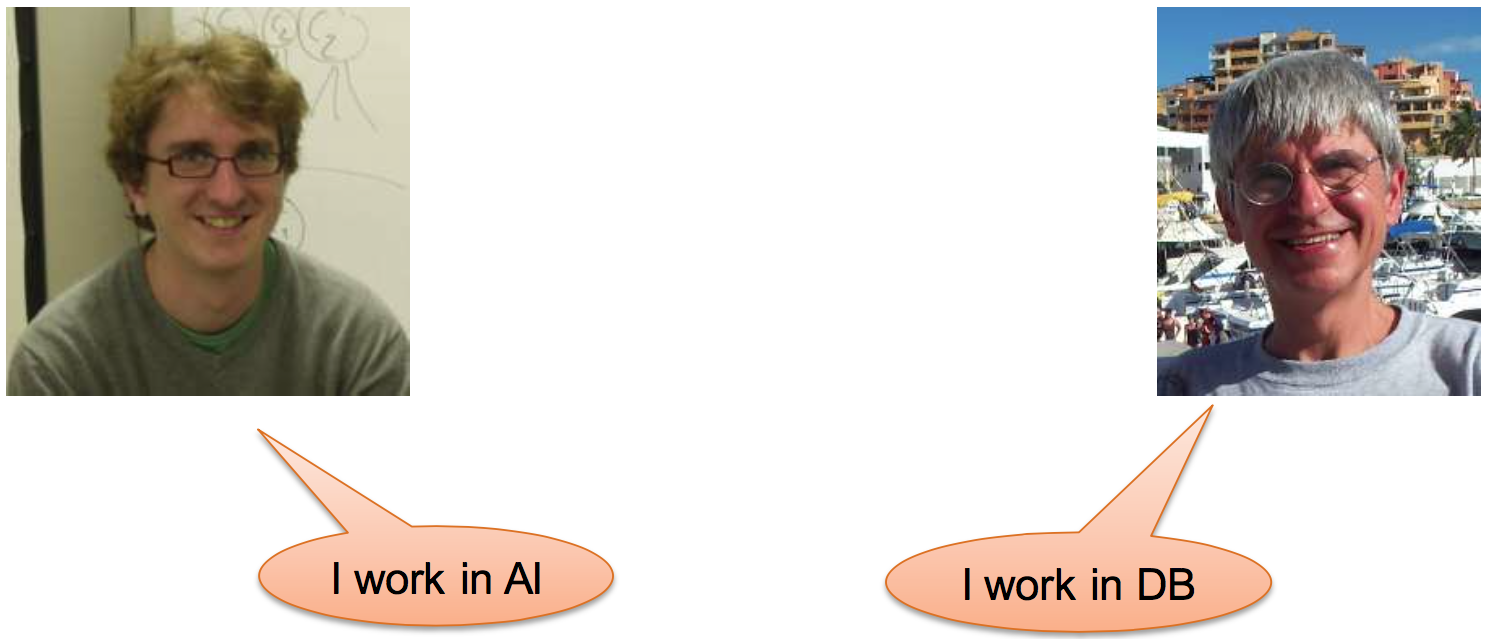
\includegraphics[width=0.91\linewidth]{authors.png}
\end{figure}

\end{frame}

\begin{frame}
\frametitle{Outline} % Table of contents slide, comment this block out to remove it
\tableofcontents 
% Throughout your presentation, if you choose to use \section{} and \subsection{} commands, these will automatically be printed on this slide as an overview of your presentation
\end{frame}

%----------------------------------------------------------------------------------------
%	PRESENTATION SLIDES
%----------------------------------------------------------------------------------------

%
%------------------------------------------------
%\section{Introduction} 
% Sections can be created in order to organize your presentation into discrete blocks, all sections and subsections are automatically printed in the table of contents as an overview of the talk
%------------------------------------------------
%
%\begin{frame}
%\frametitle{Introduction}
%\bi
%\ii \textbf{Disclaimer}
%\bi
%\ii This is not a full course on Relational Algebra
%\ii Neither this is a course on SQL
%\ei
%\ei
%
%\bi
%\ii \textbf{Introduction to Relational Algebra, RDBMS and SQL}
%\bi
%\ii Follow the video lectures of the Stanford class on RDBMS \href{https://www.coursera.org/course/db}{\texttt{https://www.coursera.org/course/db}}
%\ii Note that you have to sign up for an account 
%\ei
%\ei
%
%\bi
%\ii \textbf{Overview of this part}
%\bi
%\ii Brief introduction to simplified relational algebra
%\ii Useful to understand Pig, Hive and HBase
%\ei
%\ei
%\end{frame}
%
%------------------------------------------------
%\section{Relational Algebra Operators} 
%------------------------------------------------
%
%
%\begin{frame}
%\frametitle{Relational Algebra}
%
%\bi
%\ii \textbf{Primitives}
%\bi
%\ii Projection ($\project$)
%\ii Selection ($\select$)
%\ii Cartesian product ($\times$)
%\ii Set union ($\bigcup$)
%\ii Set difference ($-$)
%\ii Rename ($\rho$)
%\ei
%\ei
%
%\bi
%\ii \textbf{Other operations}
%\bi
%\ii Join ($\join$)
%\ii Group by ... aggregation ($\gamma$)
%\ii ...
%\ei
%\ei
%
%\end{frame}
%
%
%------------------------------------------------
%
%\begin{frame}
%\frametitle{Relational Algebra Operators}
%\bi
%\ii \textbf{There are a number of operations on data that fit well the relational algebra model}
%\bi
%\ii 􏰀In traditional RDBMS, queries involve retrieval of \myred{small amounts of data}
%􏰀\ii 􏰀 In this course, and in particular in this class, we should keep in mind the particular workload underlying MapReduce
%\ii 􏰀Full scans of large amounts of data
%\ii 􏰀Queries are not selective\footnote{This is true in general. However, most ETL jobs involve selection and projection to do data preparation.}, they process all data
%\ei
%\ei
%
%\bi
%\ii \textbf{A review of some terminology}
%\bi
%\ii 􏰀 A \myred{\textit{relation}} is a table
%\ii 􏰀 \myblue{\textit{Attributes}} are the column headers of the table
%\ii 􏰀 The set of attributes of a relation is called a \myblue{\textit{schema}}
%\ii Example: $R(A_1, A_2, ..., A_n)$ indicates a relation called $R$ whose attributes are $A_1, A_2, ..., A_n$
%\ei
%\ei
%\end{frame}
%
%------------------------------------------------
%
%\begin{frame}
%\frametitle{Operators}
%\bi
%\ii \textbf{Let’s start with an example}
%\bi
%\ii 􏰀Below, we have part of a relation called \textit{Links} describing the structure of the Web
%􏰀\ii 􏰀There are two attributes: \textit{From} and \textit{To}
%\ii 􏰀A row, or \myblue{\textit{tuple}}, of the relation is a pair of URLs, indicating the existence of a link between them
%\ii 􏰀The number of tuples in a real dataset is in the order of billions ($10^9$)
%\ei
%\ei
%
%\begin{table}[h]
%\centering
%\begin{tabular}{l l}
%\toprule
%\textbf{From} & \textbf{To}\\
%\midrule
%url1 & url2 \\
%url1 & url3 \\
%url2 & url3 \\
%url2 & url4 \\
%... & ...
%\bottomrule
%\end{tabular}
%\caption{Table caption}
%\end{table}
%
%\end{frame}
%
%------------------------------------------------
%
%\begin{frame}
%\frametitle{Operators}
%\bi
%\ii \textbf{Relations (however big) can be stored in a distributed filesystem}
%\bi
%\ii If they don't fit in a single machine, they're broken into pieces (think HDFS)
%\ei
%\ei
%\bi
%\ii \textbf{Next, we review and describe a set of relational algebra operators}
%\bi
%\ii Intuitive explanation of what they do
%\ii \textit{Pseudo-code} of their implementation in/by MapReduce
%\ei
%\ei
%\end{frame}
%
%------------------------------------------------
%
%------------------------------------------------
%
%\begin{frame}
%\frametitle{Operators}
%\bi
%\ii \textbf{Selection:} $\select_{C}(R)$
%\bi
%\ii Apply condition $C$ to each tuple of relation $R$
%\ii Produce in output a relation containing only tuples that satisfy $C$
%\ei
%\ei
%\bi
%\ii \textbf{Projection:} $\project_{S}(R)$
%\bi
%\ii Given a \textit{subset} $S$ of relation $R$ attributes
%\ii Produce in output a relation containing only tuples for the attributes in $S$
%\ei
%\ei
%\bi
%\ii \textbf{Union, Intersection and Difference} 
%\bi
%\ii Well known operators on sets
%\ii Apply to the set of tuples in two relations that have the \myblue{same schema}
%\ii Variations on the theme: work on \textit{bags}
%\ei
%
%\ei
%\end{frame}
%
%------------------------------------------------
%
%------------------------------------------------
%
%\begin{frame}
%\frametitle{Operators}
%\bi
%\ii \textbf{Natural join:} $R \join S$
%\bi
%\ii Given two relations, \textit{compare each pair of tuples}, one from each relation
%\ii If the tuples agree on all the attributes common to both schema $\rightarrow$ produce an output tuple that has components on each attribute
%\ii Otherwise produce nothing
%\ii \myred{\textit{Join condition}} can be on a subset of attributes
%\ei
%\ei
%\bi
%\ii \textbf{Let's work with an example} 
%\bi
%\ii Recall the \textit{Links} relation from previous slides
%\ii \texttt{Query} (or data processing job): \texttt{find the paths of length two in the web}
%\ei
%\ei
%\end{frame}
%
%------------------------------------------------
%
%------------------------------------------------
%
%\begin{frame}
%\frametitle{Join Example}
%\bi
%\ii \textbf{Informally, to satisfy the query we must:} 
%\bi
%\ii find the triples of URLs in the form ($u, v, w$) such that there is a link from $u$ to $v$ and a link from $v$ to $w$
%\ei
%\ei
%\bi
%\ii \textbf{Using the join operator} 
%\bi
%\ii Imagine we have two relations (with different schema), and let's try to apply the natural join operator
%\ii There are two copies of \textit{Links}: $L_1(U_1, U_2)$ and $L_2(U_2, U_3)$
%\ii Let's compute $L_1 \join L_2$
%\bi
%\ii For each tuple $t_1$ of $L_1$ and each tuple $t_2$ of $L_2$, see if their $U_2$ component are the same
%\ii If yes, then produce a tuple in output, with the schema ($U_1, U_2, U_3$)
%\ei
%\ei
%\ei
%\end{frame}
%
%------------------------------------------------
%
%------------------------------------------------
%
%\begin{frame}
%\frametitle{Join Example}
%\bi
%\ii \textbf{What we have seen is called (to be precise) a \myblue{self-join}} 
%\bi
%\ii \myred{Question:} \textit{How would you implement a self join in our favorite programming language?}
%\ii \myred{Question:} \textit{What is the time complexity of your algorithm?}
%\ii \myred{Question:} \textit{What is the space complexity of your algorithm?}
%\ei
%\ei
%\bi
%\ii \textbf{To continue the example} 
%\bi
%\ii Say you are not interested in the entire two-hop path but just the start and end nodes
%\ii Then you do a projection and the notation would be: $\project_{U_1, U_3}(L_1 \join L_2)$
%\ei
%\ei
%\end{frame}
%
%------------------------------------------------
%
%
%------------------------------------------------
%
%\begin{frame}
%\frametitle{Grouping and Aggregation Operators}
%\bi
%\ii \textbf{Grouping and Aggregation:} $\gamma_X (R)$
%\bi
%\ii The result of this operation is a relation with one tuple for each group
%\ii That tuple has a component for each of the grouping attributes, with the value common to tuples of that group
%\ii That tuple has another component for each aggregation, with the aggregate value for that group
%\ei
%\ei
%\bi
%\ii \textbf{Let's work with an example} 
%\bi
%\ii Imagine that a social-networking site has a relation \texttt{Friends(User, Friend)}
%\ii The tuples are pairs ($a, b$) such that $b$ is a friend of $a$
%\ii \texttt{Query}: \texttt{compute the number of friends each member has}
%\ei
%\ei
%\end{frame}
%
%------------------------------------------------
%
%------------------------------------------------
%
%\begin{frame}
%\frametitle{Grouping and Aggregation Operators}
%\bi
%\ii \textbf{How to satisfy the query:} $\gamma_{User, \texttt{COUNT}(Friend)} (Friends)$
%\bi
%\ii This operation groups all the tuples by the value in their first component\\ 
%$\rightarrow$ There is one group for each user
%\ii Then, for each group, it counts the number of friends
%\ei
%\ei
%\bi
%\ii \textbf{Some details} 
%\bi
%\ii The \texttt{COUNT} operation applied to an attribute does not consider the values of that attribute
%\ii In fact, it counts the number of tuples in the group
%\ii In SQL, there is a \myblue{count distinct} operator that counts the number of different values
%\ei
%\ei
%\end{frame}
%
%------------------------------------------------
%
%------------------------------------------------
%\section{Computing Relational Algebra} 
%------------------------------------------------
%
%------------------------------------------------
%
%\begin{frame}
%\frametitle{Computing Selection}
%\bi
%\ii \textbf{In practice, selections do not need a full-blown MapReduce implementation}
%\bi
%\ii They can be implemented in the \myred{map phase alone}
%\ii Actually, they could also be implemented in the reduce portion
%\ei
%\ei
%
%\bi
%\ii \textbf{A MapReduce implementation of $\select_C(R)$}
%\bi
%\ii \mygreen{\textbf{Map:}} \\
%For each tuple $t$ in $R$, check if $t$ satisfies $C$ \\
%If so, emit a key/value pair ($t, t$)
%\ii \mygreen{\textbf{Reduce:}}\\
%Identify reducer \\
%\myred{Question:} single or multiple reducers? 
%\ei
%\ei
%
%\bi
%\ii \textbf{NOTE: the output is not exactly a relation}
%\bi
%\ii \myred{WHY?}
%\ei
%\ei
%
%\end{frame}
%
%------------------------------------------------
%
%------------------------------------------------
%
%\begin{frame}
%\frametitle{Computing Projections}
%\bi
%\ii \textbf{Similar process to selection}
%\bi
%\ii But, projection may cause same tuple to appear several times
%\ei
%\ei
%
%\bi
%\ii \textbf{A MapReduce implementation of $\project_S(R)$}
%\bi
%\ii \mygreen{\textbf{Map:}} \\
%For each tuple $t$ in $R$, construct a tuple $t'$ by eliminating those components whose attributes are not in $S$ \\
%Emit a key/value pair ($t', t'$)
%\ii \mygreen{\textbf{Reduce:}}\\
%For each key $t'$ produced by any of the Map tasks, fetch, $t', [t', \cdots , t']$\\
%Emit a key/value pair ($t', t'$)
%\myred{Question:} single or multiple reducers? 
%\ei
%\ei
%
%\bi
%\ii \textbf{NOTE: the reduce operation is \myred{duplicate elimination}}
%\bi
%\ii This operation is associative and commutative, so it is possible to optimize MapReduce by using a \texttt{Combiner} in each mapper
%\ei
%\ei
%
%\end{frame}
%
%------------------------------------------------
%
%------------------------------------------------
%
%\begin{frame}
%\frametitle{Computing Unions}
%\bi
%\ii \textbf{Suppose relations $R$ and $S$ have the same schema}
%\bi
%\ii Map tasks will be assigned chunks from either $R$ or $S$
%\ii Mappers don’t do much, just pass by to reducers
%\ii Reducers do duplicate elimination
%\ei
%\ei
%
%\bi
%\ii \textbf{A MapReduce implementation of union}
%\bi
%\ii \mygreen{\textbf{Map:}}\footnote{Hadoop MapReduce supports reading multiple inputs.} \\
%For each tuple $t$ in $R$ or $S$, emit a key/value pair ($t, t$)
%\ii \mygreen{\textbf{Reduce:}}\\
%For each key $t$ there will be either one or two values\\
%Emit ($t, t$) in either case
%\ei
%\ei
%
%\end{frame}
%
%------------------------------------------------
%
%------------------------------------------------
%
%\begin{frame}
%\frametitle{Computing Intersections}
%\bi
%\ii \textbf{Very similar to computing unions}
%\bi
%\ii Suppose relations $R$ and $S$ have the same schema
%\ii The map function is the same (an identity mapper) as for union
%\ii The reduce function must produce a tuple only if both relations have that tuple
%\ei
%\ei
%
%\bi
%\ii \textbf{A MapReduce implementation of intersection}
%\bi
%\ii \mygreen{\textbf{Map:}}\\
%For each tuple $t$ in $R$ or $S$, emit a key/value pair ($t, t$)
%\ii \mygreen{\textbf{Reduce:}}\\
%If key $t$ has value list [$t, t$] then emit the key/value pair ($t, t$)\\
%Otherwise, emit the key/value pair ($t$, \texttt{NULL})
%\ei
%\ei
%
%\end{frame}
%
%------------------------------------------------
%
%------------------------------------------------
%
%\begin{frame}
%\frametitle{Computing difference}
%\bi
%\ii \textbf{Assume we have two relations $R$ and $S$ with the same schema}
%\bi
%\ii The only way a tuple $t$ can appear in the output is if it is in $R$ but not in $S$
%\ii The map function passes tuples from $R$ and $S$ to the reducer
%\ii NOTE: it must inform the reducer whether the tuple came from $R$ or $S$
%\ei
%\ei
%
%\bi
%\ii \textbf{A MapReduce implementation of difference}
%\bi
%\ii \mygreen{\textbf{Map:}}\\
%For each tuple $t$ in $R$ emit a key/value pair ($t$, '\texttt{R}') and for a tuple $t$ in $S$, emit a key/value pair ($t$, '\texttt{S}')
%\ii \mygreen{\textbf{Reduce:}}\\
%For each key $t$, do the following:\\
%If it is associated to '\texttt{R}', then emit ($t, t$) \\
%If it is associated to ['\texttt{R}', '\texttt{S}'] or ['\texttt{S}', '\texttt{R}'], or ['\texttt{S}'], emit the key/value pair ($t$, \texttt{NULL})
%\ei
%\ei
%
%\end{frame}
%
%------------------------------------------------
%\section{Join Algorihtms in MapReduce} 
%------------------------------------------------
%
%------------------------------------------------
%
%\begin{frame}
%\frametitle{Overview of SQL Joins}
%
%\begin{figure}[h]
%\centering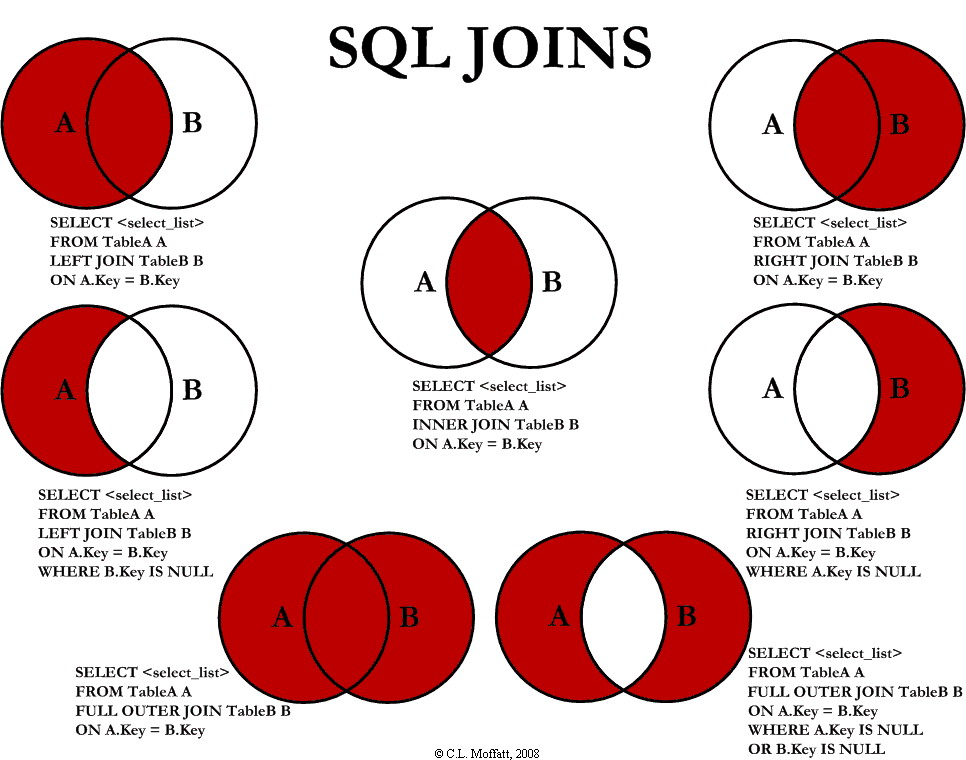
\includegraphics[width=0.91\linewidth]{sql-joins.jpg}
%\end{figure}
%
%\end{frame}
%
%------------------------------------------------
%
%------------------------------------------------
%
%\begin{frame}
%\frametitle{Join Algorihtms in MapReduce}
%
%\bi
%\ii \textbf{Reduce-side join}
%\ii \textbf{Map-side join}
%\ii \textbf{In-memory join}
%\bi
%\ii Striped variant
%\ii Memcached variant
%\ei
%\ei
%
%\end{frame}
%
%------------------------------------------------
%
%------------------------------------------------
%
%\begin{frame}
%\frametitle{Reduce-side Join}
%
%\bi
%\ii \textbf{Basic idea: group by join key}
%\bi
%\ii Map over both sets of tuples
%\ii Emit tuple as value with join key as the intermediate key
%\ii Execution framework brings together tuples sharing the same key
%\ii Perform actual join in reducer
%\ii Similar to a “sort-merge join” in database terminology
%\ei
%\ei
%
%\end{frame}
%
%------------------------------------------------
%
%------------------------------------------------
%
%\begin{frame}
%\frametitle{Map-side Join: Parallel Scans}
%
%\bi
%\ii \textbf{If datasets are sorted by join key, join can be accomplished by a scan over both datasets}
%\ei
%
%\bi
%\ii \textbf{How can we accomplish this in parallel?}
%\bi
%\ii Partition and sort both datasets in the same manner
%\ei
%\ei 
%
%\bi
%\ii \textbf{In MapReduce:}
%\bi
%\ii Map over one dataset, read from other corresponding partition
%\ii No reducers necessary (unless to repartition or resort)
%\ei
%\ei
%
%\bi
%\ii \textbf{Consistently partitioned datasets: realistic to expect?}
%\ei
%
%\end{frame}
%
%------------------------------------------------
%
%
%------------------------------------------------
%
%\begin{frame}
%\frametitle{In-Memory Join}
%
%\bi
%\ii \textbf{Basic idea: load one dataset into memory, stream over other dataset}
%\bi
%\ii Works if $R \ll S$ and $R$ fits into memory
%\ii Called a \myblue{\textit{hash join}} in database terminology
%\ei
%\ei
%
%\bi
%\ii \textbf{MapReduce implementation}
%\bi
%\ii Distribute $R$ to all nodes
%\ii Map over $S$, each mapper loads $R$ in memory, hashed by join key
%\ii For every tuple in $S$, look up join key in $R$
%\ii No reducers, unless for regrouping or resorting tuples
%\ei
%\ei
%
%\end{frame}
%
%------------------------------------------------
%
%------------------------------------------------
%
%\begin{frame}
%\frametitle{In-Memory Join: Variants}
%
%\bi
%\ii \textbf{Striped variant:}
%\bi
%\ii $R$ too big to fit into memory? 
%\ii Divide $R$ into $R_1, R_2, R_3, \cdots , R_n$ s.t. each $R_n$ fits into memory
%\ii Perform in-memory join: $\forall n, R_n \join S$
%\ii Take the union of all join results
%\ei
%\ei
%
%\bi
%\ii \textbf{Memcached join:}
%\bi
%\ii Load $R$ into memcached
%\ii Replace in-memory hash lookup with memcached lookup
%\ii \myblue{\textit{Capacity and scalability?}}
%\bi
%\ii Memcached capacity $\gg$ RAM of individual node
%\ii Memcached scales out with cluster
%\ei
%\ii \myblue{\textit{Latency?}}
%\bi
%\ii Memcached is fast (basically, speed of network)
%\ii Batch requests to amortize latency costs
%\ei
%\ei
%\ei
%
%\end{frame}
%
%------------------------------------------------
%
%------------------------------------------------
%
%\begin{frame}
%\frametitle{Which Join to Use?}
%
%\bi
%\ii \textbf{In-memory join $>$ map-side join $>$ reduce-side join}
%\bi
%\ii \myred{\textit{Why?}}
%\ei
%\ei
%
%\bi
%\ii \textbf{Limitations of each?}
%\bi
%\ii In-memory join: memory
%\ii Map-side join: sort order and partitioning
%\ii Reduce-side join: general purpose
%\ei
%\ei
%
%\end{frame}
%
%------------------------------------------------
%
%
%------------------------------------------------
%
%\begin{frame}
%\frametitle{Map-Reduce-Merge}
%
%\bi
%\ii \textbf{Map-Reduce-Merge can form a hierarchical workflow which is similar to, but much more general than a DBMS query execution plan.}
%\bi
%\ii No query operators, but arbitrary programming logic specified by the developers
%\ii More general than relational query plans
%\ii More general than Map-Reduce
%\ei
%\ei
%
%\bi
%\ii \textbf{Map:} $map(k_1, v_1) \rightarrow [(k_2, v_2)]$
%\ii \textbf{Reduce:} $reduce(k_2, [v_2]) \rightarrow [(k_2, v_3)]$
%\ii \textbf{Merge:} $merge((k_2, [v_2])_a, (k_3, [v_3])_b) \rightarrow [(k_4, v_5)]$
%\ei
%\end{frame}
%
%------------------------------------------------
%
%------------------------------------------------
%
%\begin{frame}
%\frametitle{Sort-Merge Join Algorithm}
%
%\bi
%\ii \textbf{Map:}
%\bi
%\ii Partition records into \textit{buckets} which are mutually exclusive and each key range is assigned to a \textit{Reducer}.
%\ei
%\ei
%
%\bi
%\ii \textbf{Reduce:}
%\bi
%\ii Data in the sets are merged into a \textit{sorted set} (sort the data).
%\ei
%\ei
%
%\bi
%\ii \textbf{Merge:}
%\bi
%\ii The merger \textit{joins} the sorted data for each key range.
%\ei
%\ei
%
%\textbf{MRM} allows for implementation of other join algorithms like \textit{Hash Join} and \textit{Nested Loop Join}.
%
%\end{frame}
%
%------------------------------------------------
%
%------------------------------------------------
%
%\begin{frame}
%\frametitle{Computing the natural join}
%\bi
%\ii \textbf{This topic is subject to continuous refinements}
%\bi
%\ii There are many \texttt{JOIN} operators and many different implementations
%\ii We've seen some of them in the laboratory sessions
%\ei
%\ei
%
%\bi
%\ii \textbf{Let's look at two relations $R(A, B)$ and $S(B, C)$}
%\bi
%\ii We must find tuples that agree on their $B$ components
%\ii We shall use the $B$-value of tuples from either relation as the key
%\ii The value will be the other component and the name of the relation
%\ii That way the reducer knows from which relation each tuple is coming from
%\ei
%\ei
%
%\end{frame}
%
%------------------------------------------------
%
%------------------------------------------------
%
%\begin{frame}
%\frametitle{Computing the natural join}
%
%\bi
%\ii \textbf{A MapReduce implementation of natural join}
%\bi
%\ii \mygreen{\textbf{Map:}}\\
%For each tuple $(a, b)$ of $R$ emit a key/value pair ($b$, ('\texttt{R}', $a$))\\
%For each tuple $(b, c)$ of $S$ emit a key/value pair ($b$, ('\texttt{S}', $c$))
%\ii \mygreen{\textbf{Reduce:}}\\
%Each key $b$ will be associated to a list of pairs that are either ('\texttt{R}', $a$) or ('\texttt{S}', $c$) \\
%Emit key/value pairs of the form $(b,[(a_1, b, c_1), (a_2, b, c_2), \cdots , (a_n, b, c_n)])$ 
%\ei
%\ei
%
%\bi
%\ii \textbf{NOTES}
%\bi
%\ii \myred{Question:} what if the MapReduce framework wouldn't implement the distributed (and sorted) group by?
%\ii In general, for $n$ tuples in relation $R$ and $m$ tuples in relation $S$ all with a common $B$-value, then we end up with $nm$ tuples in the result
%\ii If all tuples of both relations have the same $B$-value, then we’re computing the \textbf{Cartesian product}
%\ei
%\ei
%
%\end{frame}
%
%------------------------------------------------
%
%------------------------------------------------
%
%\begin{frame}
%\frametitle{Grouping and Aggregation in MapReduce}
%
%\bi
%\ii \textbf{Let $R(A, B, C)$ be a relation to which we apply $\gamma_{A, \theta(B)}(R)$} 
%\bi
%\ii The map operation prepares the grouping
%\ii The grouping is done by the framework
%\ii The reducer computes the aggregation
%\ii Simplifying assumptions: one grouping attribute and one aggregation function
%\ei
%\ei
%
%\bi
%\ii \textbf{A MapReduce implementation of $\gamma_{A, \theta(B)}(R)$}\footnote{Note here that we are also projecting.}
%\bi
%\ii \mygreen{\textbf{Map:}}\\
%For each tuple $(a, b, c)$ emit a key/value pair ($a, b$) \\
%\ii \mygreen{\textbf{Reduce:}}\\
%Each key a represents a group\\
%Apply $\theta$ to the list $[b_1, b_2, \cdots , b_n]$ \\
%Emit the key/value pair ($a, x$) where $x = \theta([b_1, b_2, \cdots , b_n])$
%\ei
%\ei
%
%\end{frame}
%
%------------------------------------------------
%
%------------------------------------------------
%\section{Summary} 
%------------------------------------------------
%
%------------------------------------------------
%
%\begin{frame}
%\frametitle{Summary}
%
%\bi
%\ii \textbf{MapReduce algorithms for processing relational data:}
%\bi
%\ii Group by, sorting, partitioning are handled automatically by shuffle/sort in MapReduce
%\ii Selection, projection, and other computations (e.g., aggregation), are performed either in mapper or reducer
%\ii Multiple strategies for relational joins
%\ei
%\ei
%
%\bi
%\ii \textbf{Complex operations require multiple MapReduce jobs}
%\bi
%\ii Example: top ten URLs in terms of average time spent
%\ii Opportunities for automatic optimization
%\ei
%\ei
%
%\end{frame}
%
%------------------------------------------------
%


\end{document} 